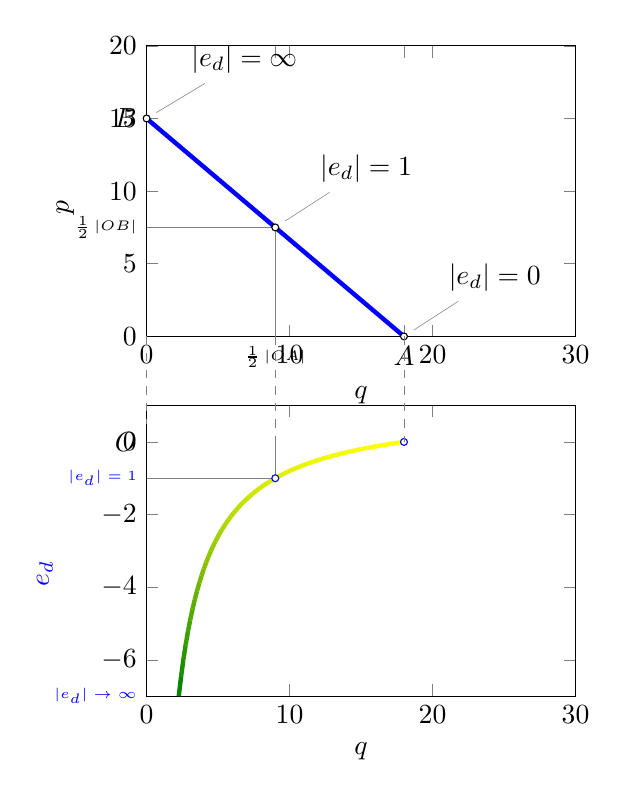
\begin{tikzpicture}
\begin{axis}[
	xmin=0,xmax=30,ymin=0,ymax=20,
	width=200pt,height=150pt,
	extra x ticks={9,18},
	extra x tick labels={{\tiny$\frac{1}{2} \left|OA\right|$},$A$},
	extra y ticks={7.5,15},
	extra y tick style={tickwidth=0},
	extra y tick labels={\tiny$\frac{1}{2} \left|OB\right|$,$B$},
	xlabel style={below},xlabel=$q$,
	ylabel style={left},ylabel=$p$,
	samples=40]
\addplot[draw=blue,domain=0:20,ultra thick] {- 5*x/6 + 15};
\node[pin=45:{$|e_d| = \infty$}] at (axis cs:0,15) {};
\node[pin=45:{$|e_d| = 1$}] at (axis cs:9,7.5) {};
\node[pin=45:{$|e_d| = 0$}] at (axis cs:18,0) {};
\addplot[gray,very thin] coordinates {(0,7.5) (9,7.5) (9,0)};	%C: ed=1
\addplot[only marks,forget plot,black,mark options={mark size=1.25pt,fill=white},mark=*] coordinates {
	(0,15)
	(9,7.5)
	(18,0)};
\coordinate (A) at (axis cs:0,0);
\coordinate (B) at (axis cs:9,0);
\coordinate (C) at (axis cs:18,0);
\end{axis}
\begin{axis}[
    extra description/.code={\node[left] at (axis cs:0,0) {$O$};},
	yshift=-130pt,colormap/greenyellow,
	xmin=0,xmax=30,ymin=-7,ymax=1,
	width=200pt,height=150pt,
	extra y ticks={-1,-7},
	extra y tick style={tickwidth=0},
	extra y tick labels={\tiny\textcolor{blue}{$|e_d| = 1$},\tiny\textcolor{blue}{$|e_d| \rightarrow \infty$}},
	xlabel style={below},xlabel=$q$,
	ylabel style={left},ylabel=\textcolor{blue}{$e_d$},
	samples=40]
\addplot[draw=blue,domain=2.25:18,ultra thick,mesh,samples=100] {-(18/x)+1};
\addplot[only marks,forget plot,blue,mark options={mark size=1.25pt,fill=white},mark=*] coordinates {
	(9,-1)
	(18,0)};
\addplot[gray,very thin] coordinates {(0,-1) (9,-1) (9,0)};	%C: ed=1
\coordinate (AN) at (axis cs:0,0.5);
\coordinate (BN) at (axis cs:9,0);
\coordinate (CN) at (axis cs:18,0);
\end{axis}
\draw[gray,very thin,dashed] (A) -- (AN);
\draw[gray,very thin,dashed] (B) -- (BN);
\draw[gray,very thin,dashed] (C) -- (CN);
\end{tikzpicture}